\documentclass[11pt,table]{article}
\usepackage{jeffe,handout}
\usepackage{fancyvrb}
\usepackage{tikz}
\usepackage{pgfkeys}
\usepackage{array,relsize}
%\usepackage[shortlabels,inline]{enumitem}
\usepackage[shortlabels,inline]{enumitem}
\newcolumntype{E}{>{\centering\arraybackslash}p{9mm}}
\newcolumntype{P}{>{\centering\arraybackslash}p{5mm}}
\newcolumntype{Q}{>{\centering\arraybackslash}p{2mm}}
\newcommand{\elide}[1]{}

\usepackage{multicol}
\newcommand{\marksamt}[1]{\textbf{[#1~marks]}}
\newcommand{\markamt}[1]{\textbf{[#1~mark]}}
\newcommand{\fillinMC}[1]{\fillinMCmath{\mbox{#1}}}
\newcommand{\fillinMCmath}[1]{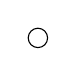
\begin{tikzpicture}\draw circle [radius=0.35em];\end{tikzpicture}\ #1}

\newcommand{\filledMC}[1]{\filledMCmath{\mbox{#1}}}
\newcommand{\filledMCmath}[1]{
\begin{tikzpicture}\draw[fill=black] circle [radius=0.35em];\end{tikzpicture}\ #1}

\newcommand{\fillinMCAll}[1]{\fillinMCAllmath{\mbox{#1}}}
\newcommand{\fillinMCAllmath}[1]{\begin{tikzpicture}\draw (0,0) rectangle (1em,1em);\end{tikzpicture}\ #1}
\newcommand{\fillinblank}[1]{\fillinblankmath{\mbox{#1}}}
\newcommand{\fillinblankmath}[1]{\begingroup\setlength{\fboxsep}{1em}\setlength{\fboxrule}{2pt}\fbox{\LARGE\phantom{#1}}\endgroup}


\newcommand{\filledblank}[1]{\filledblankmath{#1}}
\newcommand{\filledblankmath}[1]{\begingroup\setlength{\fboxsep}{1em}\setlength{\fboxrule}{2pt}\fbox{\LARGE{#1}}\endgroup}

\newcommand{\filledSblank}[1]{\filledSblankmath{#1}}
\newcommand{\filledSblankmath}[1]{\begingroup\setlength{\fboxsep}{1em}\setlength{\fboxrule}{2pt}\fbox{#1}\endgroup}

\newcommand{\fillbox}[3]{%
% #1 : width
% #2 : height
% #3 : contents
\sbox{0}{\parbox{#1}{\rule{0pt}{0pt}\LARGE{#3}}}%
\ifdim\dimexpr\ht0+\dp0<#2% 
\dp0\dimexpr#2-\ht0\fi%
\begingroup\setlength{\fboxsep}{1em}\setlength{\fboxrule}{2pt}%
\fbox{\usebox{0}}%
\endgroup%
}


\newcommand{\blank}{\rule{3mm}{0.1mm}}
\newcommand{\blankk}{\rule{2cm}{0.1mm}}
\newcommand{\shade}{\cellcolor[gray]{0.8}}

%\def\rmdefault{bch} % Use Charter for main text font.
\usepackage{tikz}
\usepackage{tikz-qtree}
\usetikzlibrary{shapes.geometric}

\usepackage{forest}

\forestset{%
subtri/.style={isosceles triangle,draw,shape border rotate=90,minimum size=.7cm,child anchor=apex,anchor=apex}
}



% definitions for formatting code blocks
\usepackage{listings}
%\usepackage{color}
\definecolor{dkgreen}{rgb}{0,0.6,0}
\definecolor{gray}{rgb}{0.5,0.5,0.5}
\definecolor{mauve}{rgb}{0.58,0,0.82}

\lstset{frame=tb,
  language=C++,
  aboveskip=3mm,
  belowskip=3mm,
  showstringspaces=false,
  columns=flexible,
  basicstyle={\small\ttfamily},
  numbers=left,
  numberstyle=\tiny\color{gray},
  keywordstyle=\color{blue},
  commentstyle=\color{dkgreen},
  stringstyle=\color{mauve},
  breaklines=true,
  breakatwhitespace=true,
  tabsize=3
}

% end definitions for formatting code blocks

\def\BOX#1{\fbox{\vbox to #1{\vss\hbox to #1{\hss}}}}
\def\Bigbox{\BOX{0.25in}}
\def\Bigbox{\raisebox{-0.5ex}[0.25in][0pt]{\BOX{0.25in}}}
\def\problem#1{\def\problemheading{#1}\clearpage\item{\bf #1.}}

\hidesolutions

\renewcommand{\arraystretch}{2}

% =========================================================
\begin{document}

\headers{CPSC 221}{ }{Winter 1, 2019}

\begin{center}
    \LARGE
    \textbf{Assignment 3}
    \\[1ex]
    \Large Due 23:59, Friday, November 15, 2019 \\
\end{center}

\begin{table}[h]
    \centering
    \renewcommand{\arraystretch}{1.5}
    \begin{tabular}{ll}
%        \textbf{Name}: & \\
%        \textbf{Student ID}: & \\
        \textbf{CS ID 1}: & \textbf{d6a2b}\\
        \textbf{CS ID 2}: & \textbf{z0n1b}\\
    \end{tabular}
\end{table}

\textbf{Instructions:}
\begin{enumerate}
\item Do not change the problem statements we are giving you. Simply add your solutions by editing this latex document. 
\item Take as much space as you need for each problem. You'll tell us where your solutions are when you submit your paper to gradescope. 
\item Export the completed assignment as a PDF file for upload to gradescope.
\item On gradescope, upload only \textbf{one} copy per partnership. (Instructions for uploading to gradescope will be posted on the HW2 page of the course website.)
\end{enumerate}

\newpage
\begin{enumerate}

\newcommand{\I}{\ensuremath{\mathit{I}}}
\renewcommand{\O}{\ensuremath{\mathit{O}}}
\renewcommand{\E}{\ensuremath{\mathit{E}}}
\newcommand{\D}{\ensuremath{\mathit{D}}}

\problem{AVL tree height: a tighter upper bound (30 points)}

We all know that AVL trees with $n$ nodes have height $O(\log n)$ but what exactly is the best upper bound on their height?
In class, we saw that height is no more than $2 \lg n$ (here $\lg$ means $\log_2$), but we know that's a little loose.
\begin{enumerate}
\item (3 points)
In class, we started with a recurrence for the function $N(h)$ which is the fewest number of nodes that an AVL tree of height $h$ can have.
Write that recurrence here:

$N(0)=$ \fillbox{1cm}{5mm}{%
% your answer here
1
}
$N(1)=$ \fillbox{1cm}{5mm}{%
% your answer here
2
}

$N(h)=$ \fillbox{7cm}{5mm}{%
% your answer here
N(h-1)+N(h-2)+1
}

\item (5 points)
Draw a smallest (with fewest nodes) AVL tree of height $h$ for $h=2,3,4$.
One for $h=5$ has magically shown up on this page!

\begin{center}
\begin{tabular}{ccc}
\fillbox{15mm}{25mm}{%
% your answer here
\includegraphics[width=15mm]{q1-h2.png}
}
&
\fillbox{25mm}{35mm}{%
% your answer here
\includegraphics[width=25mm]{q1-h3.png}
}
&
\fillbox{35mm}{45mm}{%
% your answer here
\includegraphics[width=35mm]{q1-h4.png}
}
\\
$h=2$&$h=3$&$h=4$
\end{tabular}\\

\begin{forest}
for tree={inner sep=2pt,fill,draw,circle,l sep-=1em,l-=1em}
  [[[[[[][,phantom]][]][[][,phantom]]][[[][,phantom]][]]][[[[][,phantom]][]][[][,phantom]]]]
\end{forest}\\
$h=5$
\end{center}

\item (5 points)
The Fibonacci numbers obey the recurrence:
$F(0) = 0$, $F(1)=1$, and $F(h)=F(h-1)+F(h-2)$.
That's so close to $N(h)$, maybe we can use it!

What are $N(h)$ and $F(h)$ for the following values of $h$:

\begingroup
\setlength{\tabcolsep}{0pt}
\begin{tabular}{rcccccccc}
&$h=0$&$1$&$2$&$3$&$4$&$5$&$6$&$7$\\
$N(h)$~~&
\fillbox{2em}{1em}{%
% answer here
1
} &
\fillbox{2em}{1em}{%
% answer here\
2
} &
\fillbox{2em}{1em}{%
% answer here
4
} &
\fillbox{2em}{1em}{%
% answer here
7
} &
\fillbox{2em}{1em}{%
% answer here
12
} &
\fillbox{2em}{1em}{%
% answer here
20
} &
\fillbox{2em}{1em}{%
% answer here
33
} &
\fillbox{2em}{1em}{%
% answer here
54
}\\
$F(h)$~~&\fillbox{2em}{1em}{%
% answer here
0
} &
\fillbox{2em}{1em}{%
% answer here
1
} &
\fillbox{2em}{1em}{%
% answer here
1
} &
\fillbox{2em}{1em}{%
% answer here
2
} &
\fillbox{2em}{1em}{%
% answer here
3
} &
\fillbox{2em}{1em}{%
% answer here
5
} &
\fillbox{2em}{1em}{%
% answer here
8
} &
\fillbox{2em}{1em}{%
% answer here
13
}\\
\end{tabular}
\endgroup

Express the relation that you observe as an equation using the functions $N()$ and $F()$.
Consider the difference between $N(h)$ and $F(h+c)$ for some constant $c$.

\fillbox{6cm}{5mm}{%
% answer here
N(h)=F(h+3)-1
}\\

\item (5 points)
Prove that the relation is correct using the recurrence that defines $F(h)$ and the recurrence that defines $N(h)$ from part (a).

\hrulefill

% answer here
Reminders of recurrences from part a:
\\N(h)=N(h-1)+N(h-2)+1
\\F(h)=F(h-1)+F(h-2)
\\
\\Inductive proof: Base case is h=2
\\Using recurrence from part a:
\\N(h=0)=1, N(h=1)=2
\\N(h=2)=N(h-2)+N(h-1)+1=1+2+1=4
\\Using hypothesized equation:
\\N(h=2)=F(h+3)-1=F(h=2+3)+1=F(5)-1=5-1=4
\\
\\Inductive hypothesis: Assume hypothesized equation is true for all h=h-1,h-2...2
\\Induction step:
\\N(h)=N(h-2)+N(h-1)+1
\\=[F((h-2)+3)-1]+[F((h-1)+3)-1]+1
\\=[F((h-2)+3)+F((h-1)+3)]+[-1-1+1]
\\=[F(h+2) + F(h+1)] -1
\\=F(h+3)-1
\\

\item (5 points)
Suppose we guess that $F(h)$ is increasing exponentially.
In other words, $F(h) = x^h$.
What could $x$ be?
We know $F(h) = F(h-1)+F(h-2)$ so it must be that
$x^h = x^{h-1} + x^{h-2}$.
For $x \neq 0$, by dividing both sides by $x^{h-2}$, we see that this is equivalent to $x^2 = x + 1$.
What two values of $x$ satisfy this equation? (You might need to remember the quadratic formula for solving this.)

\hrulefill

% answer here
$x^2 = x + 1$
\\$x^2-x-1 = 0$
\\The quadratic formula is $x=\frac{-b\pm\sqrt{b^2-4ac}}{2a}$. 
In this case a=1, b=-1, c=-1 
\\so the x that satisfies the equation are:

\\x1=(1+sqrt(5))/2
\\x2=(1-sqrt(5))/2
\\

\item (2 points)
If $r$ is the positive and $s$ is the negative solution that you found,
then $F(h) = r^h$ and $F(h)= s^h$ both satisfy $F(h)=F(h-1)+F(h-2)$, but they don't satisfy $F(0)=0$ and $F(1)=1$.
However, we can create more functions that satisfy $F(h)=F(h-1)+F(h-2)$ by mixing these two solutions. For example, any function $a r^h + b s^h$ for numbers $a$ and $b$ also satisfies $F(h)=F(h-1)+F(h-2)$.
For what values of $a$ and $b$ does this mixture satisfy $F(0)=0$ and $F(1)=1$?

$a=$ \fillbox{5cm}{5mm}{%
% answer here
1/sqrt(5)
}

$b=$ \fillbox{5cm}{5mm}{%
% answer here
-1/sqrt(5)
}
 
 
\item (5 points)
The result of the previous derivation implies (after a bit of work) that 
$\displaystyle F_{h}=\left\lfloor {\frac {\varphi ^{h}}{\sqrt {5}}}+{\frac {1}{2}}\right\rfloor
>
\varphi^h / \sqrt{5} - 1$,
where $\varphi = (1+\sqrt{5})/2 \approx 1.618$ is the golden ratio.
Use this expression for $F(h)$ along with the answer to part (c) to show that every AVL tree with $n$ nodes has height $h < p \log_2 (n + 2) + q$ for some constants $p$ and $q$.
What are those constants?
Show your work.

\hrulefill

$p=$ \fillbox{6cm}{5mm}{%
% answer here
$\displaystyle 1/log_{2}(\varphi)$
}

$q=$ \fillbox{6cm}{5mm}{%
% answer here
$\displaystyle log_{\varphi}(\sqrt{5})-3$
}

% Show your work here
N(h)=F(h+3)-1
\\N(h)+1=F(h+3)
\\N(h)+1$\displaystyle >\varphi^{h+3} / \sqrt{5} - 1$
\\$\displaystyle \sqrt{5}(N+2) > \varphi^{h+3}$
\\$\displaystyle h + 3 < log_{\varphi}(\sqrt{5}(N+2))$
\\$\displaystyle h < log_{\varphi}(N+2)+log_{\varphi}(\sqrt{5}) - 3$
\\$\displaystyle h < log_{2}(N+2)/log_{2}(\varphi)+log_{\varphi}(\sqrt{5}) - 3$

\end{enumerate}



\problem{Binary search tree split and join (25 points)}

Suppose we would like to support the operation \textbf{split} which takes a (pointer to a) binary search tree $T$ and a key $k$ and splits the tree $T$ into two binary search trees $L$ and $R$.
All the nodes in $T$ with key $\leq k$ go into $L$ and the others go into $R$.
The key $k$ may or may not be in the tree $T$.

\begin{enumerate}
\item (2 points)
Circle all the nodes and subtrees that should end up in tree $L$ after splitting the following binary search tree using key $k$.

%\begin{center}
%\begin{forest}
%for tree={circle,draw,inner sep=0pt,l-=1ex,l sep-=1ex,s sep+=2ex,minimum size=.5cm,edge=-latex,anchor=north}
%[$x_1$[$x_2$[$L_2$,subtri][$x_3$[$x_4$[$k$[$L_5$,subtri][$R_5$,subtri]][$R_4$,subtri]][$R_3$,subtri]]][$R_1$,subtri]]
%\end{forest}
%\end{center}

\includegraphics[width=50mm]{q2-a.png}

\item (4 points)
Draw the two trees $L$ and $R$ resulting from the split of the previous tree using key $k$.
You should use the nodes and subtrees
of the previous tree in your solution.

Remember that both $L$ and $R$ must be binary search trees.

\hrulefill

% answer here
\includegraphics[width=100mm]{q2-b.png}

\vspace{10cm}

\end{enumerate}

Of course, we would also like to be able to split an AVL tree $T$ in the same fashion so that the resulting trees $L$ and $R$ are AVL trees.
This is more complicated.
We can't simply do what we did for part (b) since the resulting trees may not have the balance property.
However, recall that all subtrees of an AVL tree are themselves AVL trees.
We can use this fact to come up with an efficient method to restructure what we did for part (b) into two AVL trees.



Interestingly, a key ingredient of the procedure to split AVL trees is a procedure to \textbf{join} two AVL trees $T_1$ and $T_2$ into one AVL tree $T$ given that the keys in $T_1$ are smaller than the keys in $T_2$.
Suppose the $\text{height}(T_1) \geq \text{height}(T_2)$; the other case is symmetric.

The first step of \textbf{join} is to find a key $x$ in $T_2$, called the \textbf{join key}, that can serve as the parent of both a subtree $A$ in $T_1$ and the AVL tree $T_2$ with $x$ removed.

\begin{enumerate}[resume]

\item (2 points)
For this configuration to obey the search tree property, what relation is $x$ to the other keys in $T_2$?

\fillbox{0.9\linewidth}{2cm}{%
% Your answer goes here
x is the smallest key in T2, since x has to be parent to both A (which is subtree of T1) and T2, and keys in T1 are smaller than keys in T2.
}

\item (2 points)
What relation is $x$ to the keys in $A$?

\fillbox{0.9\linewidth}{2cm}{%
% Your answer goes here
x is larger than all keys in A.
}

\end{enumerate}

Let $T'_2$ be the tree $T_2$ after $x$ is removed.
The idea is to identify a subtree $A$ in $T_1$ that could be the sibling of $T'_2$ in the joined AVL tree. Then replace $A$ with
tree
\[
B= \begin{forest}
for tree={circle,draw,inner sep=0pt,l-=1ex,l sep-=1ex,s sep+=2ex,minimum size=.5cm,edge=-latex,anchor=north}
[$x$[$A$,baseline,subtri][$T'_2$,subtri]]
\end{forest}
\]
where $x$ is the appropriate key (from part (c)) removed from $T_2$.
For this to work, we need the tree obtained by replacing $A$ with $B$ in $T_1$ to be an AVL tree.

\begin{enumerate}[resume]
\item (2 points)
What condition must be true of the height of $A$ if $h$ is the height of $T'_2$?


\fillbox{6cm}{1.5cm}{%
% Your answer goes here
Height of A has to be h-1, h, or h+1.
}

\item (2 points)
Where can we find the root of an appropriate subtree $A$ in $T_1$ so that the search tree ordering is preserved after the replacement?

\fillbox{0.9\linewidth}{2cm}{%
% Your answer goes here
Start with root of A being root of T1, and keep traversing right (increasing order) in T1 using root of A until A's height is h2+1 (minimum traversal along T1). (Note that you may need to rotate tree afterwards if A has the +1 that keeps the tree barely balanced, so adding x in will unbalance the tree)
}

\item (4 points)
How many nodes do you need to visit to find an appropriate subtree $A$ in $T_1$ as a function of the heights $h_1$ of $T_1$ and $h_2$ of $T'_2$?  Don't worry about additive constants.

\fillbox{3cm}{1cm}{%
% Your answer goes here
h1-(h2+1)
}


\end{enumerate}

We are now prepared to split an AVL tree $T$ using a key $k$ into two AVL trees $L$, containing keys that are $\leq k$, and $R$, containing keys that are $> k$.
The first step is the same as for general binary search trees: Find the path of nodes $P = x_1, x_2, \dots, x_m$ from the root $x_1$ of $T$ to the key $x_m=k$ or to the parent $x_m$ of the position where $k$ would be inserted.
Notice that I'm using the key value to specify the node.
A node $x_i$ on this path typically has one child that is not on the path.
If this child is a left child of $x_i$, we call its subtree $L_i$.
If it's a right child of $x_i$, we call its subtree $R_i$.
If $x_m=k$ then the key $k$ is in tree $T$ and any children of $k$ are not on the path and their subtrees are called $L_m$ (for a left child) and $R_m$ (for a right child).
If $x_m \neq k$ then the key $k$ is not in tree $T$ and $x_m$ has at most one child which is called $L_m$ (for a left child) or $R_m$ (for a right child).
See the figure in part (a) for an example of this type of labeling when $x_m = k$.

For this example, to create $R$, we join $R_5$ with $R_4$ using $x_4$ as the join key.
We then join the resulting AVL tree, called $R_5 x_4 R_4$, with $R_3$ using $x_3$ as the join key.
Finally, we join $R_5 x_4 R_4 x_3 R_3$ to $R_1$ using $x_1$ as the join key.


\begin{enumerate}[resume]

\item (5 points)
How much time does it take in the worst case to create $R$ following this scheme when we start with an AVL tree that contains $n$ nodes?
Use asymptotic notation to express your answer.
For full credit, briefly explain your answer.


\fillbox{0.9\linewidth}{4cm}{%
% Your answer goes here
If worst case is xh=k (best case is x0=k) and h is function of log(n), we need to reattach log(n) amount of right subtrees, so worst case time is O(log(n)). Note that in worst case, all reattaching would need rebalancing, but since rebalancing is O(1), we can ignore it.
}


\item (2 points)
How would you create the AVL tree containing node $k$ and subtree $L_5$ that will then be joined with $L_2$ using $x_2$ as the join key?

\fillbox{0.9\linewidth}{2cm}{%
% Your answer goes here
Put k to rightmost in L5. Rebalance as needed. Then, attach L5 to right of x2. Rebalance as needed. Although you need to traverse L5 to drop off k, this method ensures balance (and AVL-ness).
}

\end{enumerate}

\problem{Deque and Fill (14 points)}

In PA2, you used a vector to implement a deque that doesn't allow elements to be added on the left.
To avoid wasting too much space at the beginning of the vector, you occasionally need to \textbf{downsize}, that is, move the $k$ pieces of data from the vector into a new empty vector of size $k$.  The details are described in the assignment and quoted below:


\begin{quote}
\sffamily
You will write a class named Deque which is a modification of a doubly ended queue structure. While the standard deque allows for insertion and removal at both ends of a contiguous arrangement of data, our deque will allow insertion and removal at one end, but only removal at the other. For convenience, we will refer to the removal-only end as the left end, and the other as the right.

Your deque should be implemented as follows: The underlying data structure will be a C++ standard vector. Following the convention of the queue we discussed in class, you will allow the data to ``float'' in the vector, with the following difference: If, upon a removal, you discover that the contiguous block of data (whose size is, say, $k$) will ``fit'' in the first $k$ positions of the vector, then you should resize down by making a new vector and copying the $k$ pieces of data into that new vector using the \texttt{push\_back} function. Additions to the structure can use the standard vector functions, and can only occur at the ``right'' side of the contiguous data (i.e. the position of largest index). (Note that in this implementation the structure is not ``circular'' - we do not wrap the data using the modulo of the array size.)
\end{quote}

\begin{enumerate}
\item (6 points)
Explain why executing a sequence of $n$ operations using this implementation of the deque takes total time $O(n)$.

\fillbox{0.9\linewidth}{15cm}{%
% Your answer goes here
If you have to copy, it means that current empty size is equals to current filled size, which means that current filled size is half of original filled size. If you suppose original filled size is $n=2^k$, then current filled size would $=(2^k)/2=2^{(k-1)}$, which is also the number of copies you have to make to fill in the empty space. Since you want to shrink every time filled size is halved, you would have to copy $=2^{(k-1)}+2^{(k-2)}+...+2^0$ times by the time all items are removed. Sum of that series $=(2^k-1)=(n-1)$=O(n), so executing a sequence of n operations takes total of O(n) time.
}

\item (2 points)
What assumptions do you make about the cost of vector operations in C++ (including vector's resize capability)?

\fillbox{0.9\linewidth}{5cm}{%
% Your answer goes here
Copying individual members of array and resizing the array both takes O(1) to execute. 
}

\end{enumerate}

We used this deque structure to help calculate the Voronoi diagram associated with an image.
Given an image of $W \times H$ pixels and a set of $C$ centers (i.e., pixels in the image), we want to color all pixels with the color of their closest center.


\begin{center}
\includegraphics[width=6cm]{park.png}
\includegraphics[width=6cm]{bfssolidparkbig.png}\\
In this example, $W=582$, $H=437$, and $C=29$.
\end{center}

\begin{enumerate}[resume]
\item (2 points)
One way to produce these diagrams is to loop over all pixels in the image and for each pixel calculate the closest center to the pixel and then color it with the center's color.
If we used this approach (without doing anything fancy), what would be its asymptotic time complexity to calculate the Voronoi diagram of an image of $W \times H$ pixels with $C$ centers?

\fillbox{4cm}{1cm}{%
% Your answer goes here
O(WHC)
}

\item (2 points)
Instead, in the programming assignment, we used a deque to support a breadth-first fill of the image starting from each center.
What is the asymptotic running time of this Voronoi fill algorithm as a function of $W$, $H$, and $C$?

\fillbox{4cm}{1cm}{%
% Your answer goes here
O(WH)
}

\item (2 points)
If $n$ is the number of pixels in the image and we choose $C$ to be a constant fraction of $n$, what are the asymptotic running times of option (c) and option (d) as functions of $n$?

Option (c):
\fillbox{4cm}{1cm}{%
% Your answer goes here
O(n^3)
}

Option (d):
\fillbox{4cm}{1cm}{%
% Your answer goes here
O(n^2)
}




\end{enumerate}

\end{enumerate}
\newpage
%----------------------------------------------------------------------
Blank sheet for extra work.




\end{document}
